\documentclass[letterpaper, 10 pt,onecolumn]{article}

\usepackage[papersize={8.5in,11.in},text={7.5in,9.75in}]{geometry}

\usepackage{graphics}
\usepackage{graphicx} % For including and formatting image files
\usepackage{multirow}
\usepackage{longtable}
\usepackage{epsfig}
\usepackage{epstopdf}

\usepackage{amsmath, mathrsfs, dsfont}
\usepackage{amssymb}
\usepackage{amsfonts}
\usepackage{bm}


\usepackage{cite}
\usepackage{verbatim}

\usepackage{amscd}
\usepackage{color}
\definecolor{lgray}{gray}{0.6}
\usepackage{rotating}


%\usepackage[font=footnotesize]{caption}
%\usepackage[caption=false,font=footnotesize]{subfig}
\usepackage[font=footnotesize]{subcaption}

\usepackage{mathptmx}
\usepackage[11pt]{moresize}
\usepackage{flushend}
\usepackage[stable]{footmisc}

\usepackage{algorithmicx}
\usepackage{algorithm}
\usepackage{algpascal}
\usepackage{float}
\usepackage{algc}
\usepackage{algcompatible}
\usepackage{algpseudocode}

\renewcommand{\algorithmicrequire}{\textbf{Input:}}  % Use Input in the format of Algorithm  
\renewcommand{\algorithmicensure}{\textbf{Output:}} % Use Output in the format of Algorithm  
\usepackage[vcentermath]{youngtab} % For typesetting Young Tableaux
\usepackage{url}
%\usepackage{breakurl}   
            

%-----------------------------------------%
% Define custom symbols
\newcommand{\BoldA}				{ \mathbf{A} }
\newcommand{\Bolda}				{ \mathbf{a} }
\newcommand{\BoldB}				{ \mathbf{B} }
\newcommand{\Boldb}				{ \mathbf{b} }
\newcommand{\BoldC}				{ \mathbf{C} }
\newcommand{\Boldc}				{ \mathbf{c} }
\newcommand{\BoldD}				{ \mathbf{D} }
\newcommand{\Boldd}				{ \mathbf{d} }
\newcommand{\BoldE}				{ \mathbf{E} }
\newcommand{\Bolde}				{ \mathbf{e} }
\newcommand{\BoldF}				{ \mathbf{F} }
\newcommand{\BoldG}				{ \mathbf{G} }
\newcommand{\g}					{ \mathbf{g} }
\newcommand{\BoldH}				{ \mathbf{H} }
\newcommand{\Boldh}				{ \mathbf{h} }
\newcommand{\BoldI}				{ \mathbf{I} }
\newcommand{\I}					{ \mathbf{I} }
\newcommand{\BoldJ}				{ \mathbf{J} }
\newcommand{\BoldK}				{ \mathbf{K} }
\newcommand{\Boldk}				{ \mathbf{k} }
\newcommand{\BoldM}				{ \mathbf{M} }
\newcommand{\BoldN}				{ \mathbf{N} }
\newcommand{\Boldn}				{ \mathbf{n} }
\newcommand{\BoldO}				{ \mathbf{O} }
\newcommand{\BoldP}				{ \mathbf{P} }
\newcommand{\Boldp}				{ \mathbf{p} }
\newcommand{\BoldQ}				{ \mathbf{Q} }
\newcommand{\Boldq}				{ \mathbf{q} }
\newcommand{\BoldR}				{ \mathbf{R} }
\newcommand{\R}					{ \mathbf{R} }
\newcommand{\Boldr}				{ \mathbf{r} }
\newcommand{\Bolds}				{ \mathbf{s} }
\newcommand{\BoldS}				{ \mathbf{S} }
\newcommand{\BoldT}				{ \mathbf{T} }
\newcommand{\BoldU}				{ \mathbf{U} }
\newcommand{\Boldu}				{ \mathbf{u} }
\newcommand{\BoldV}				{ \mathbf{V} }
\newcommand{\Boldv}				{ \mathbf{v} }
\newcommand{\Boldw}				{ \mathbf{w} }
\newcommand{\BoldW}				{ \mathbf{W} }
\newcommand{\BoldX}				{ \mathbf{X} }
\newcommand{\Boldx}				{ \mathbf{x} }
\newcommand{\BoldY}				{ \mathbf{Y} }
\newcommand{\Boldy}				{ \mathbf{y} }
\newcommand{\BoldZ}				{ \mathbf{Z} }
\newcommand{\Boldz}				{ \mathbf{z} }


\newcommand{\0}					{ \boldsymbol{0} }
\newcommand{\1}					{ \boldsymbol{1} }

\newcommand{\dtheta}			{ \delta\boldsymbol{\theta} }
\newcommand{\noiseg}			{ \mathbf{n}_{g} }
\newcommand{\noisewg}			{ \mathbf{n}_{{\omega}g} }
\newcommand{\noisea}			{ \mathbf{n}_{a} }
\newcommand{\noisewa}			{ \mathbf{n}_{{\omega}a} }
\newcommand{\Boldomega}			{ \boldsymbol{\omega} }
\newcommand{\Boldnu}			{ \boldsymbol{\nu} }
\newcommand{\BoldGamma}			{ \boldsymbol{\Gamma} }
\newcommand{\Boldgamma}			{ \boldsymbol{\gamma} }
\newcommand{\Boldkappa}			{ \boldsymbol{\kappa} }
\newcommand{\BoldPhi}			{ \boldsymbol{\Phi} }
\newcommand{\Boldphi}			{ \boldsymbol{\phi} }
\newcommand{\Boldpi}			{ \boldsymbol{\pi} }
\newcommand{\Boldrho}			{ \boldsymbol{\rho} }
\newcommand{\Boldell}			{ \boldsymbol{\ell} }
%\newcommand{\0}					{ \boldsymbol{0} }
\newcommand{\Bolddelta}			{ \boldsymbol{\delta} }
\newcommand{\BoldDelta}			{ \boldsymbol{\Delta} }
\newcommand{\BoldTheta}			{ \boldsymbol{\Theta} }
\newcommand{\Boldtheta}			{ \boldsymbol{\theta} }
\newcommand{\BoldSigma}			{ \boldsymbol{\Sigma} }
\newcommand{\Boldsigma}			{ \boldsymbol{\sigma} }
\newcommand{\Boldeps}			{ \boldsymbol{\epsilon} }
\newcommand{\Boldmu}			{ \boldsymbol{\mu} }
\newcommand{\Boldeta}			{ \boldsymbol{\eta} }
\newcommand{\Boldzeta}			{ \boldsymbol{\zeta} }
\newcommand{\Boldlambda}		{ \boldsymbol{\lambda} }
\newcommand{\BoldLambda}		{ \boldsymbol{\Lambda} }
\newcommand{\Boldchi}			{ \boldsymbol{\chi} }

\newcommand{\E}					{\mathrm{E}}
\newcommand{\Var}				{\mathrm{Var}}
\newcommand{\Cov}				{\mathrm{Cov}}
\newcommand\norm[1]{\lVert#1\rVert}

\newcommand\T{\rule{0pt}{2.6ex}}       % Top strut
\newcommand\B{\rule[-1.2ex]{0pt}{0pt}} % Bottom strut

\newcounter{inlineenum}
\renewcommand{\theinlineenum}{\alph{inlineenum}}
\newenvironment{inlineenum}
{\unskip\ignorespaces\setcounter{inlineenum}{0}%
	\renewcommand{\item}{\refstepcounter{inlineenum}{\textit{\theinlineenum})~}}}

\newcommand{\icol}[1]{% inline column vector
	\left(\begin{matrix}#1\end{matrix}\right)%
}
\newcommand{\irow}[1]{% inline row vector
	\begin{matrix}(#1)\end{matrix}%
}

%-----------------------------------------%
% Define custom operators
\DeclareMathOperator*{\argmin}{\emph{arg\,min}}

%-----------------------------------------%
% Define custom commands
%\newcommand{\or}{\bf or}
%\newcommand{\and}{\bf and}
\newtheorem{Theorem}{Theorem}[section]
\newtheorem{Proposition}[Theorem]{Proposition}
\newtheorem{Lemma}[Theorem]{Lemma}
\newtheorem{Corollary}[Theorem]{Corollary}
\newtheorem{Remark}[Theorem]{\textbf{Remark}}
	\newcommand{\brmrk}[1]{\begin{remark} \label{#1} }
	\newcommand{\ermrk}{ \hfill $\bigtriangleup$    \end{remark} \vspace{1mm} }
\newtheorem{Definition}[Theorem]{Definition}
\newtheorem{Example}[Theorem]{Example}
\newtheorem{Conjecture}[Theorem]{Conjecture}
\newtheorem{Problem}[Theorem]{Problem}
\newtheorem{Algorithm}[Theorem]{Algorithm}
\newtheorem{CardGame}[Theorem]{Card Game}
\newtheorem{Strategy}[Theorem]{Strategy}
\newtheorem{Question}[Theorem]{Question}
\newtheorem{exercise}{Exercise}[section]
\newcommand{\boex}[1]{\begin{example} \label{#1} --- \rm}
	\newcommand{\eoex}{ \hfill $\bigtriangleup$    \end{example} \vspace{1mm} }
\newtheorem{example}{Example}[section]
\newcommand{\bohw}[1]{\begin{exercise} \label{#1} -- \rm}
	\newcommand{\eohw}{ \hfill    \end{exercise} \vspace{1mm} }
\newtheorem{assumption}{Assumption}[section]
	\newcommand{\boass}[1]{\begin{assumption} \label{#1} -- \rm}
	\newcommand{\eoass}{ \hfill    \end{assumption} \vspace{1mm} }

\newcommand{\todo}[1]{\footnote{\color{green}TO DO: {#1}}}

\newcommand{\tstamp}{\today}
%\usepackage{fancyhdr}
%\pagestyle{fancy}
%\headheight 35pt

%\rhead{\tstamp}
%\chead{Middle top}
%\lhead{Left top}
%\rfoot{p. \thepage}
%\cfoot{}
%\lfoot{Copyright \textcopyright 2019, University of California, Riverside. All Rights reserved.}

\renewcommand{\baselinestretch}{1.0}

\setcounter{secnumdepth}{3}
\setcounter{tocdepth}{2}

\newcommand{\black}{\color{black}}
\newcommand{\blue}{\color{blue}}
\newcommand{\red}{\color{red}}
\newcommand{\green}{\color{green}}
\newcommand{\magenta}{\color{magenta}}
\newcommand{\cyan}{\color{cyan}}
\definecolor{brinkpink}{rgb}{1.00, 0.33, 0.64}
\newcommand{\pink}{\color{brinkpink}}

%\newcommand{\black}{\color{black}}
%\newcommand{\blue}{\color{black}}
%\newcommand{\red}{\color{black}}
%\newcommand{\green}{\color{black}}
%\newcommand{\magenta}{\color{black}}

\makeatletter
\newenvironment{breakablealgorithm}
{% \begin{breakablealgorithm}
	\begin{center}
		\refstepcounter{algorithm}% New algorithm
		\hrule height.8pt depth0pt \kern2pt% \@fs@pre for \@fs@ruled
		\renewcommand{\caption}[2][\relax]{% Make a new \caption
			{\raggedright\textbf{\ALG@name~\thealgorithm} ##2\par}%
			\ifx\relax##1\relax % #1 is \relax
			\addcontentsline{loa}{algorithm}{\protect\numberline{\thealgorithm}##2}%
			\else % #1 is not \relax
			\addcontentsline{loa}{algorithm}{\protect\numberline{\thealgorithm}##1}%
			\fi
			\kern2pt\hrule\kern2pt
		}
	}{% \end{breakablealgorithm}
		\kern2pt\hrule\relax% \@fs@post for \@fs@ruled
	\end{center}
}
\makeatother








\usepackage{acro}
\begin{document}
	\title{Experiment Analysis Support Document}
	\author{Wang~Hu,
		and~Jay~A.~Farrell
	}
	\maketitle
	
	
	This support document provides additional information related those experiments that could not fit within the page constraints of VN-DGNSS paper \cite{hu2021using}.
	
	\section{Stationary test}
	
	For the stationary test, all the receivers were connected to a high quality antenna mounted on the roof of Winston Chung Hall at the University of California, Riverside. That antenna location was determined by Online Positioning User Service (OPUS). This antenna is located on the roof of Winston Chung Hall at the University of California, Riverside. The antenna has a clear view of the open sky. The elevation angle cutoff for all receivers was set to 15$^\circ$. For a long duration test, to analyze position estimation accuracy, UTC time, geodetic and geocentric coordinates were saved using u-center software. The underlying u-blox raw data (e.g., measurements, satellite status) were not saved.
	
	
	\section{Moving test}
	
	For the moving tests, the raw data was stored as `.ubx' files using u-center software. The data files are available in the `test\_data' folder at the open-source repository\footnote{VN-DGNSS repository: \url{https://github.com/Azurehappen/Virtual-Network-DGNSS-Project}.}. The files are named according to the acronyms defined in Table IV of the paper \cite{hu2021using}. The files that are named as `RTK' are those for which the receiver was operating ground truth trajectory. The elevation angle cutoff for all 4 receivers was set to 15$^\circ$. During the experiment, the u-blox RTK status always maintained integer fixed solution indicating that it had centimeter accuracy.
	
	\subsection{Vehicle Trajectories}	
	
	Fig. \ref{fig:trj_mt1} and Fig. \ref{fig:trj_mt2} show the vehicle trajectory for the moving test using single-band and dual-band antenna, respectively.
	Since the receivers were all connected to the same antenna, the effects on the experiment of the surroundings (e.g., mountains, buildings, foliage) are the same for all receivers. 
	\begin{figure}[H]
		\centering
		\hfill
		\begin{subfigure}{.45\textwidth}
			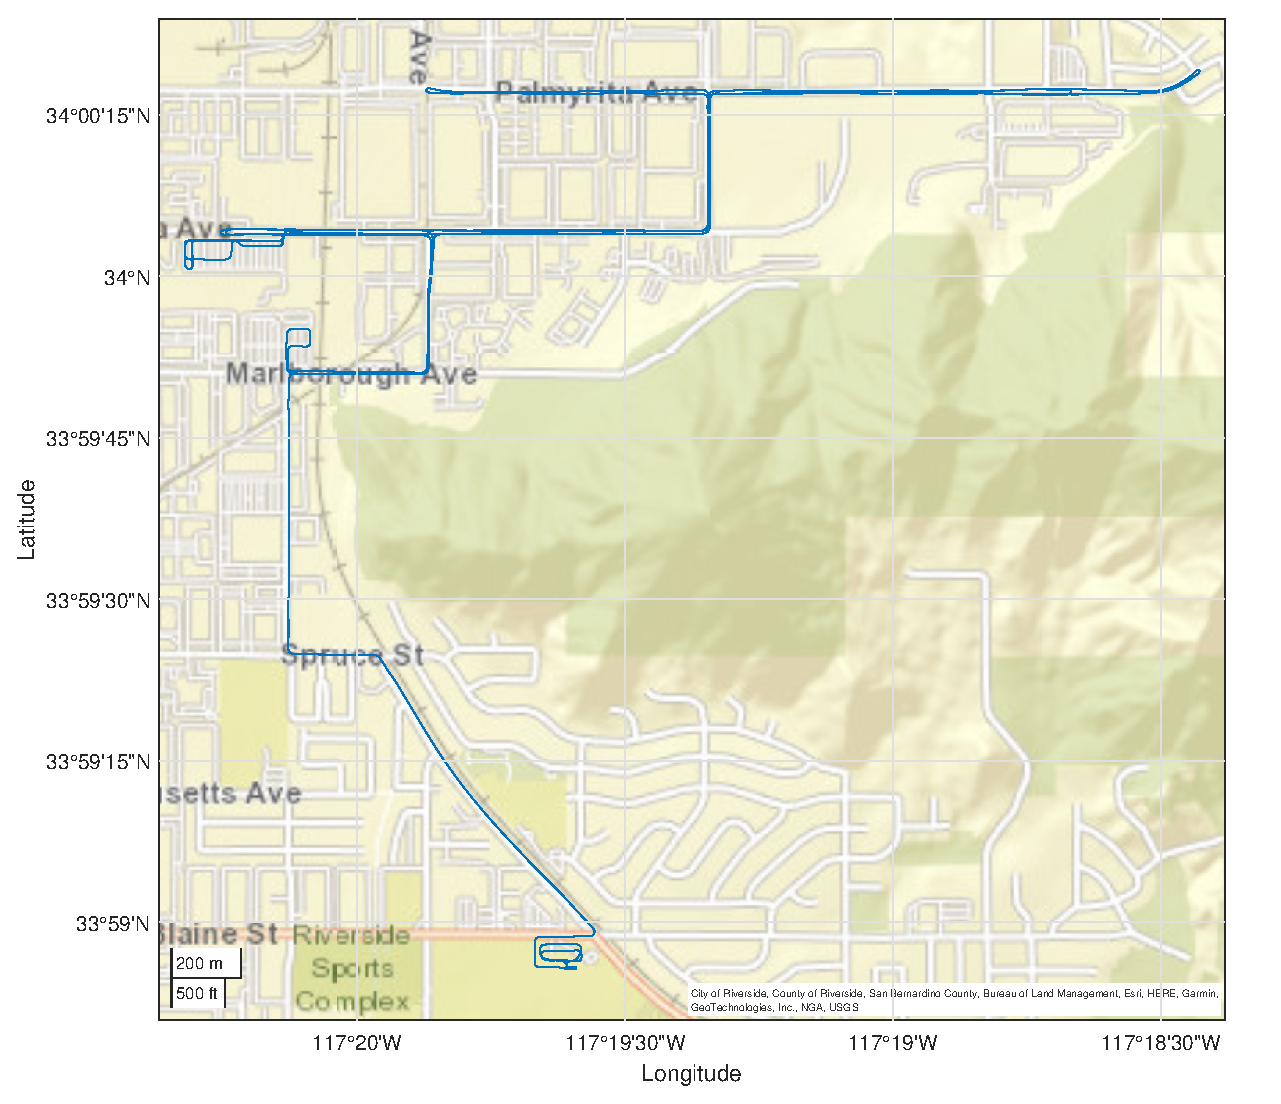
\includegraphics[width=\linewidth]{figures/trajectory_single.eps}
			\caption{Vehicle trajectory during the moving test using the single band antenna.}
			\label{fig:trj_mt1}
		\end{subfigure}%
		\hfill
		\begin{subfigure}{.45\textwidth}
			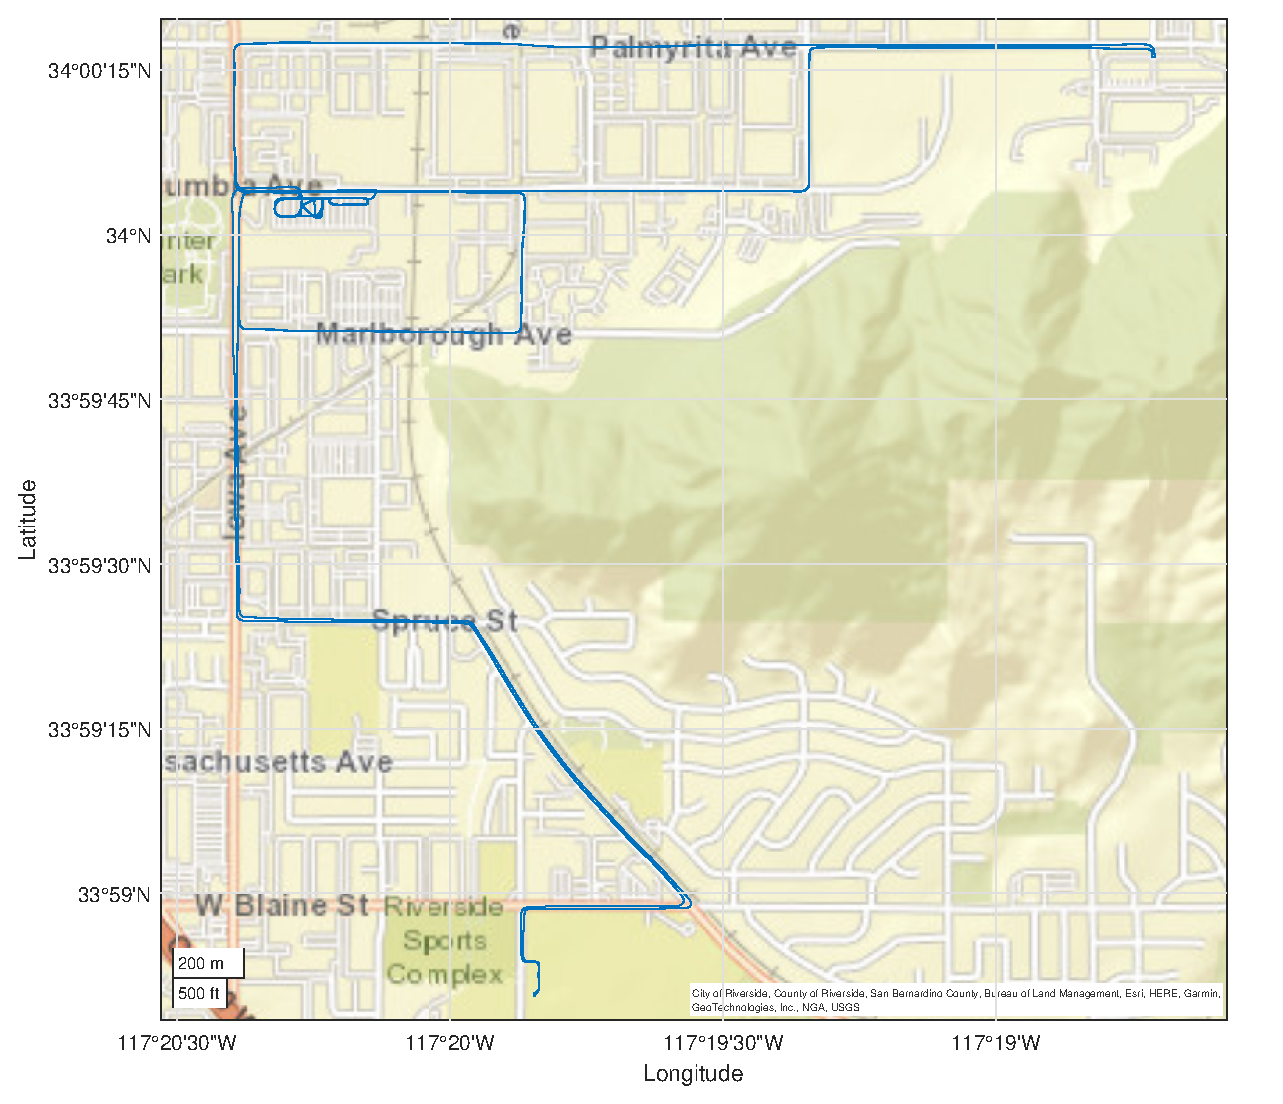
\includegraphics[width=\linewidth]{figures/trajectory_dual.eps}
			\caption{Vehicle trajectory during the moving test using the dual band antenna.}
			\label{fig:trj_mt2}
		\end{subfigure}
		\hfill
		\caption[short]{Vehicle trajectories during the moving test.}
		\label{fig:trj}
	\end{figure}%
	
	
	
	
	
	\subsection{Satellite Sky Plots}
	
	The sky plots in Fig. \ref{fig:mt1} and \ref{fig:mt2} show the satellites that were tracked during the F9P SBAS experiment. 
	Fig. \ref{fig:mt1_sky} and Fig. \ref{fig:mt2_sky} show the sky plots with satellite ID marking its final location. 
	Each satellite includes a system  identifier: 
	`G' stands for GPS, 
	`E' stands for Galileo, 
	`B' stands for BeiDou. \blue 
	The number following the system identifier is the satellite PRN. \black
	\red 
	The receivers using the VN-DGNSS approach do not use SBAS satellites. 
	The receiver performing RTK did not use SBAS and Galileo satellites because u-blox M8P does not support them.
	\black
	
	Fig. \ref{fig:mt1_obt} and Fig. \ref{fig:mt2_obt} more clearly show each satellite orbit, without the satellite ID. 
	Green indicates those satellite  used in navigation. 
	Cyan indicates satellites whose signal was available but not used because their elevation is \red lower than the elevation that user set. \black
	Blue indicates satellites whose signal was available but not use in navigation for other reasons. 
	Red  indicates satellites whose signal is not available. 
	Several reasons will cause blue or red \cite{ucenter}, e.g.: unhealthy status reported by satellite, lack of ephemeris, low signal strength, below the elevation cutoff angle. 
	%
	The orbits for some satellites, such as B21, E5, and G24, change colors in Figs. \ref{fig:mt1}.
	This means that their available or unavailable status changed during the time interval of the experiment.
	For example, when a satellite is at a low elevation and rising, it may switch from unavailable to available. 
	\begin{figure}[b]
		\centering
		\begin{subfigure}{.45\textwidth}
			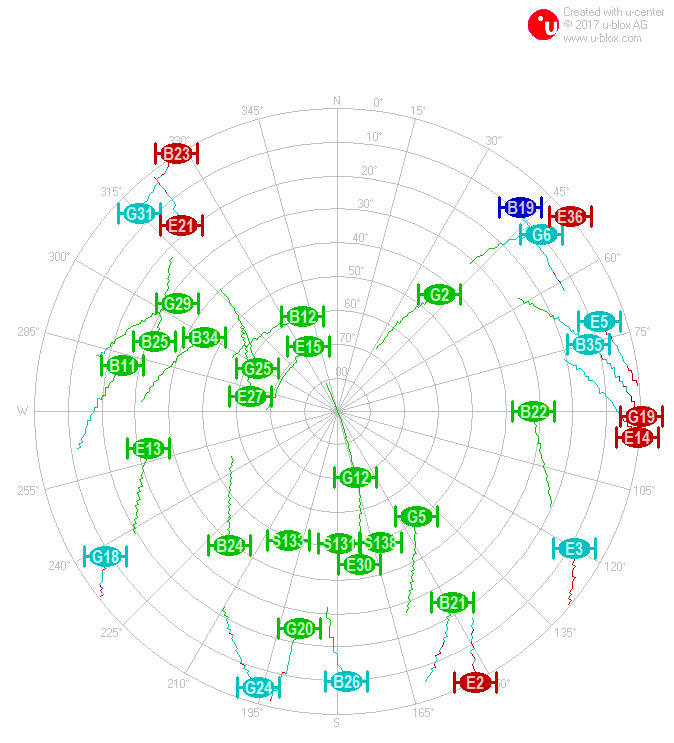
\includegraphics[width=\linewidth]{../Moving_SingleBand/skyplot.png}
			\caption{With satellite ID.}
			\label{fig:mt1_sky}
		\end{subfigure}%
		\hfill
		\begin{subfigure}{.45\textwidth}
			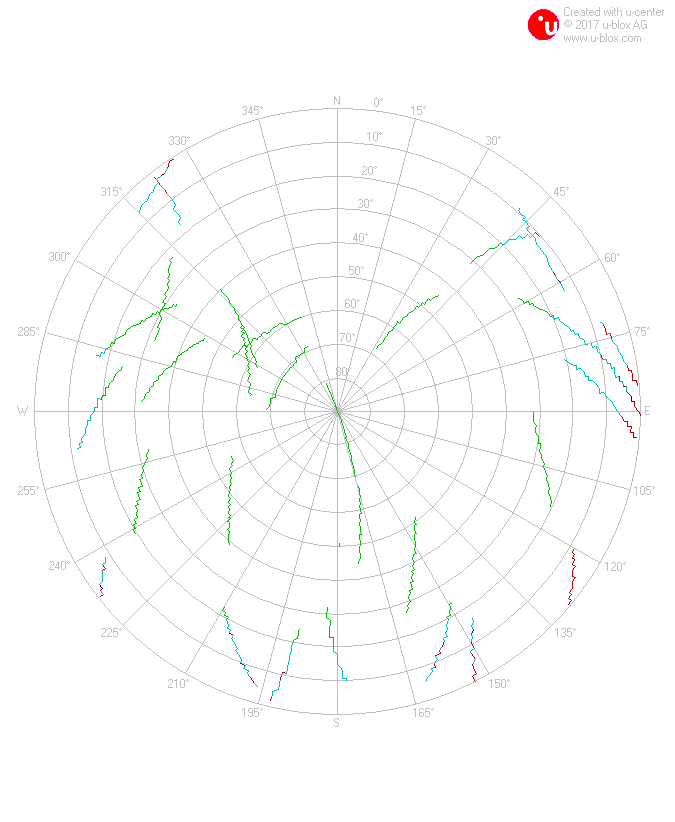
\includegraphics[width=\linewidth]{../Moving_SingleBand/skyplot_orbit.png}
			\caption{	Without satellite ID.}
			\label{fig:mt1_obt}
		\end{subfigure}
		\caption[short]{Sky plot and satellite orbit during the moving test that used the single band antenna.}
		\label{fig:mt1} 
	\end{figure}
	\begin{figure}[tb]
		\centering
		\begin{subfigure}{.5\textwidth}
			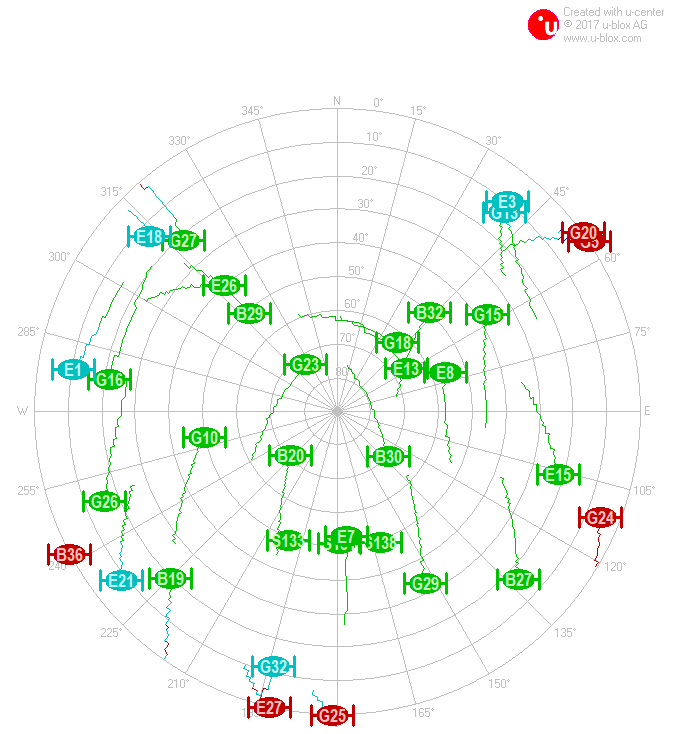
\includegraphics[width=0.9\linewidth]{../Moving_DualBand/skyplot.png}
			\caption{	
				With satellite ID.}
			\label{fig:mt2_sky}
		\end{subfigure}%
		\hfill
		\begin{subfigure}{.5\textwidth}
			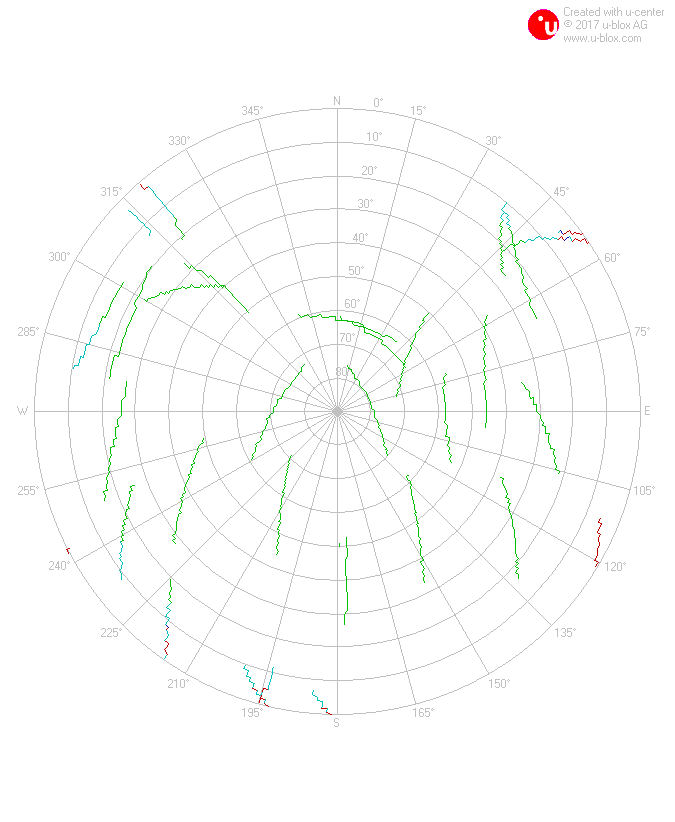
\includegraphics[width=0.9\linewidth]{../Moving_DualBand/skyplot_orbit.png}
			\caption{	
				Without satellite ID.}
			\label{fig:mt2_obt}
		\end{subfigure}
		\caption[short]{Sky plot and satellite orbit during moving test that used the dual band antenna.}
		\label{fig:mt2}
	\end{figure}
	
	\subsection{Vehicle Speed, Number of Satellites, and Signal Quality during the Moving Tests}
	
	Fig. \ref{fig:m1vspeed}a and Fig. \ref{fig:m2vspeed}a show the horizontal position error relative to the RTK ground truth trajectory as discussed in Section VI.D of \cite{hu2021using}. 
	Fig. \ref{fig:m1vspeed}b and Fig. \ref{fig:m2vspeed}b show the vehicle speed over ground as \red reported by the receiver using RTK. \black
	
	Fig. \ref{fig:m1vspeed}c and Fig. \ref{fig:m2vspeed}c show the number of satellites used in the navigation solution for each of the experimental configurations listed  by acronyms in Table IV of \cite{hu2021using}. 
	%
	The number of satellites per experimental configuration are similar, and always more than sufficient to yield a good GDOP, but have minor variations. 
	The purple line in Fig. \ref{fig:m1vspeed}c shows that the SF GNSS OS, F9P SBAS, SF GNSS VN configurations all use the same number of satellites. 
	These numbers do not count for the SBAS satellites since they provides corrections, but are not used for positioning.
	The number of satellites used in RTK is less than others is because the u-blox M8P does not support the Galileo system.
	
	The reason that the number of satellites change is satellite signal loss. 
	The attached video shows an example of the satellite information interface from the u-center during rerun of the moving test data from the F9P SBAS experiment. 
	The following definitions are required to support the discussion:
	\begin{itemize}
		\item The column `Qi' is the signal quality indicator. 
		The values of `Qi' are defined in Table \ref{tab:qi}. 
		Each satellite will only be used for pseudorange positioning  when $Qi \geq 4$. 
		Use of carrier data for RTK, requires $Qi = 7$.
		\item The `PR used' indicate that if the satellite code measurement is used, Y for yes and N for no.
	\end{itemize}
	When a satellite's signal fades, is blocked by obstructions, or a cycle slip is detected \cite{sennott1992use},  the receiver may change the signal quality indicator  to code unlocked statuses ($Qi = 0,1,2,3$). 
	Fig. \ref{fig:qi} and the attached video show the Qi of satellite E3 was dropped from 7 to 0 when the signal was lost.
	Then, the Qi changes back to 7 when the receiver re-locks the satellite. 
	In Fig. \ref{fig:qi}b, satellite E3 is not used when $Qi \geq 4$, which explains the change in the total number of satellites used as shown in Fig. \ref{fig:qi}a.
	
	
	
	\begin{table}[H]
		\centering
		\begin{tabular}{|c|c|c|}
			\hline
			Value & Description                                   & Additional remarks                 \\ \hline
			0     & no signal                                     &                                    \\ \hline
			1     & searching signal                              &                                    \\ \hline
			2     & signal acquired                               &                                    \\ \hline
			3     & signal detected but unusable                  &                                    \\ \hline
			4     & code locked and time synchronized             &                                    \\ \hline
			5     & code and carrier locked and time synchronized & carrier lock has not been achieved \\ \hline
			6     & code and carrier locked and time synchronized & carrier lock is intermittent       \\ \hline
			7     & code and carrier locked and time synchronized & carrier lock achieved              \\ \hline
		\end{tabular}
		\caption{Definition of signal quality indicator}
		\label{tab:qi}
	\end{table}
	\clearpage
	
	\begin{figure}[H]
		\centering
		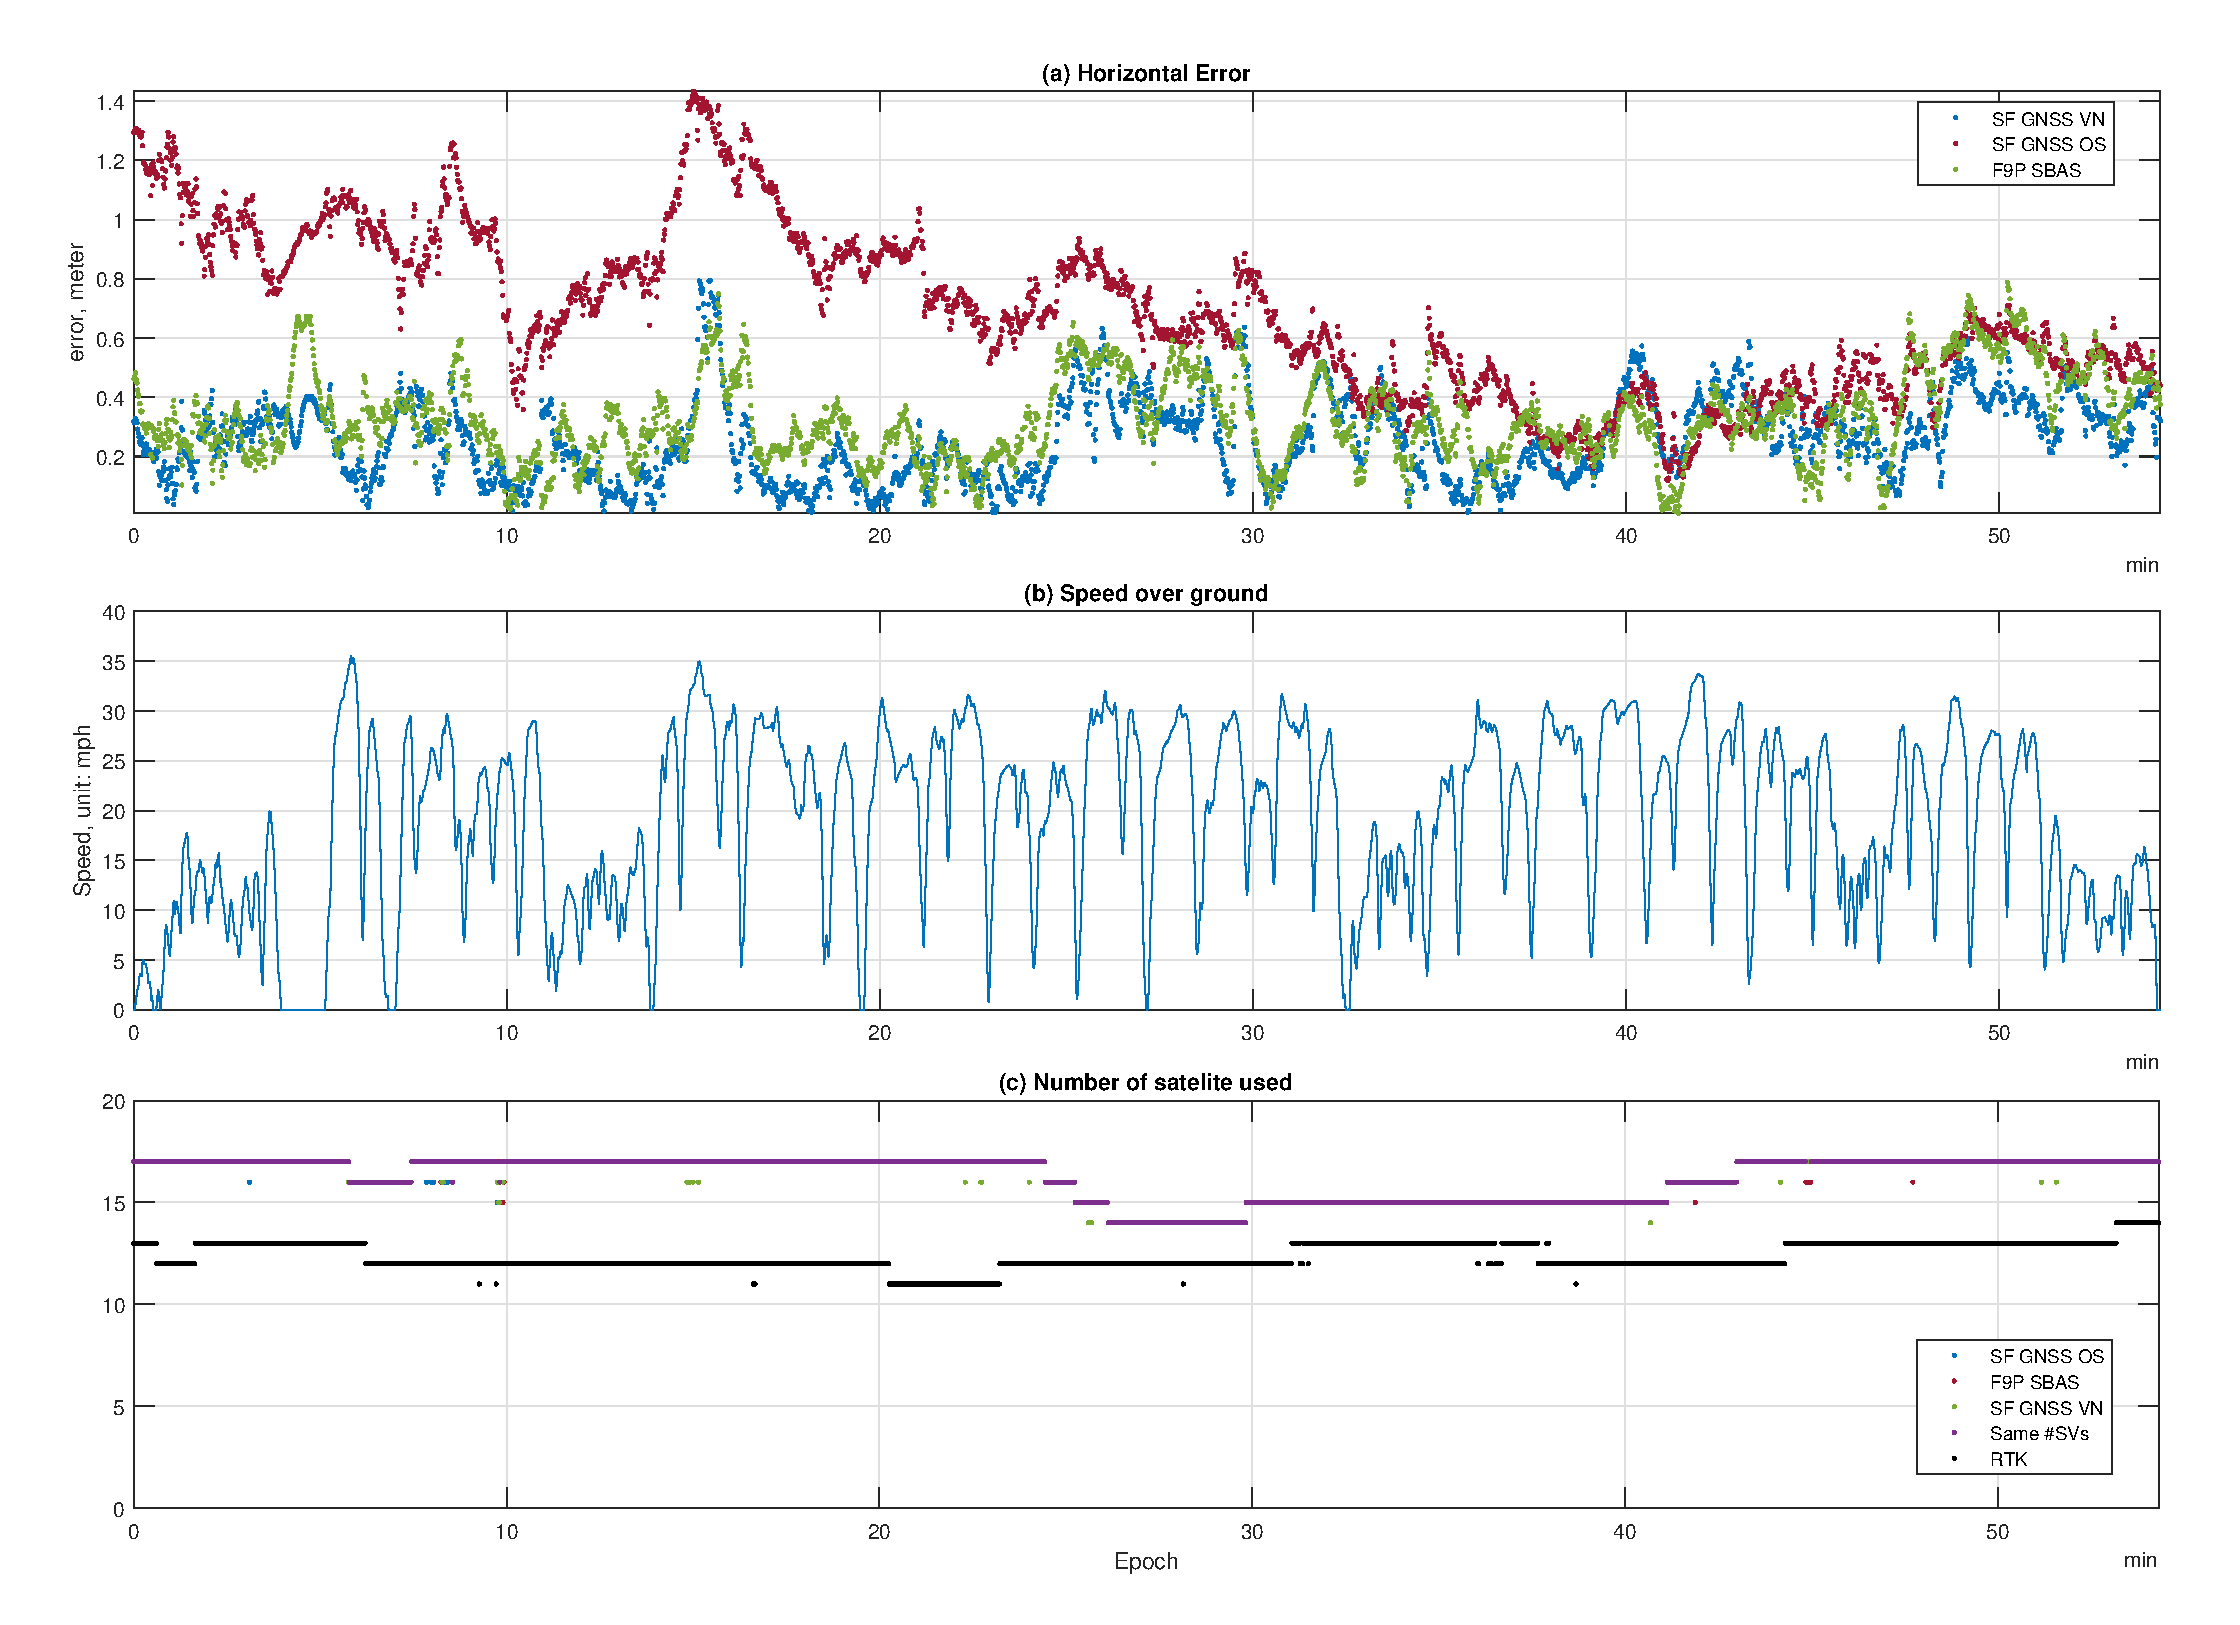
\includegraphics[width=0.9\textwidth]{figures/dynamicinfo_single.eps}
		\caption{Vehicle speed and number of satellites used for moving test using single band antenna.}
		\label{fig:m1vspeed}
	\end{figure}
	
	\begin{figure}[H]
		\centering
		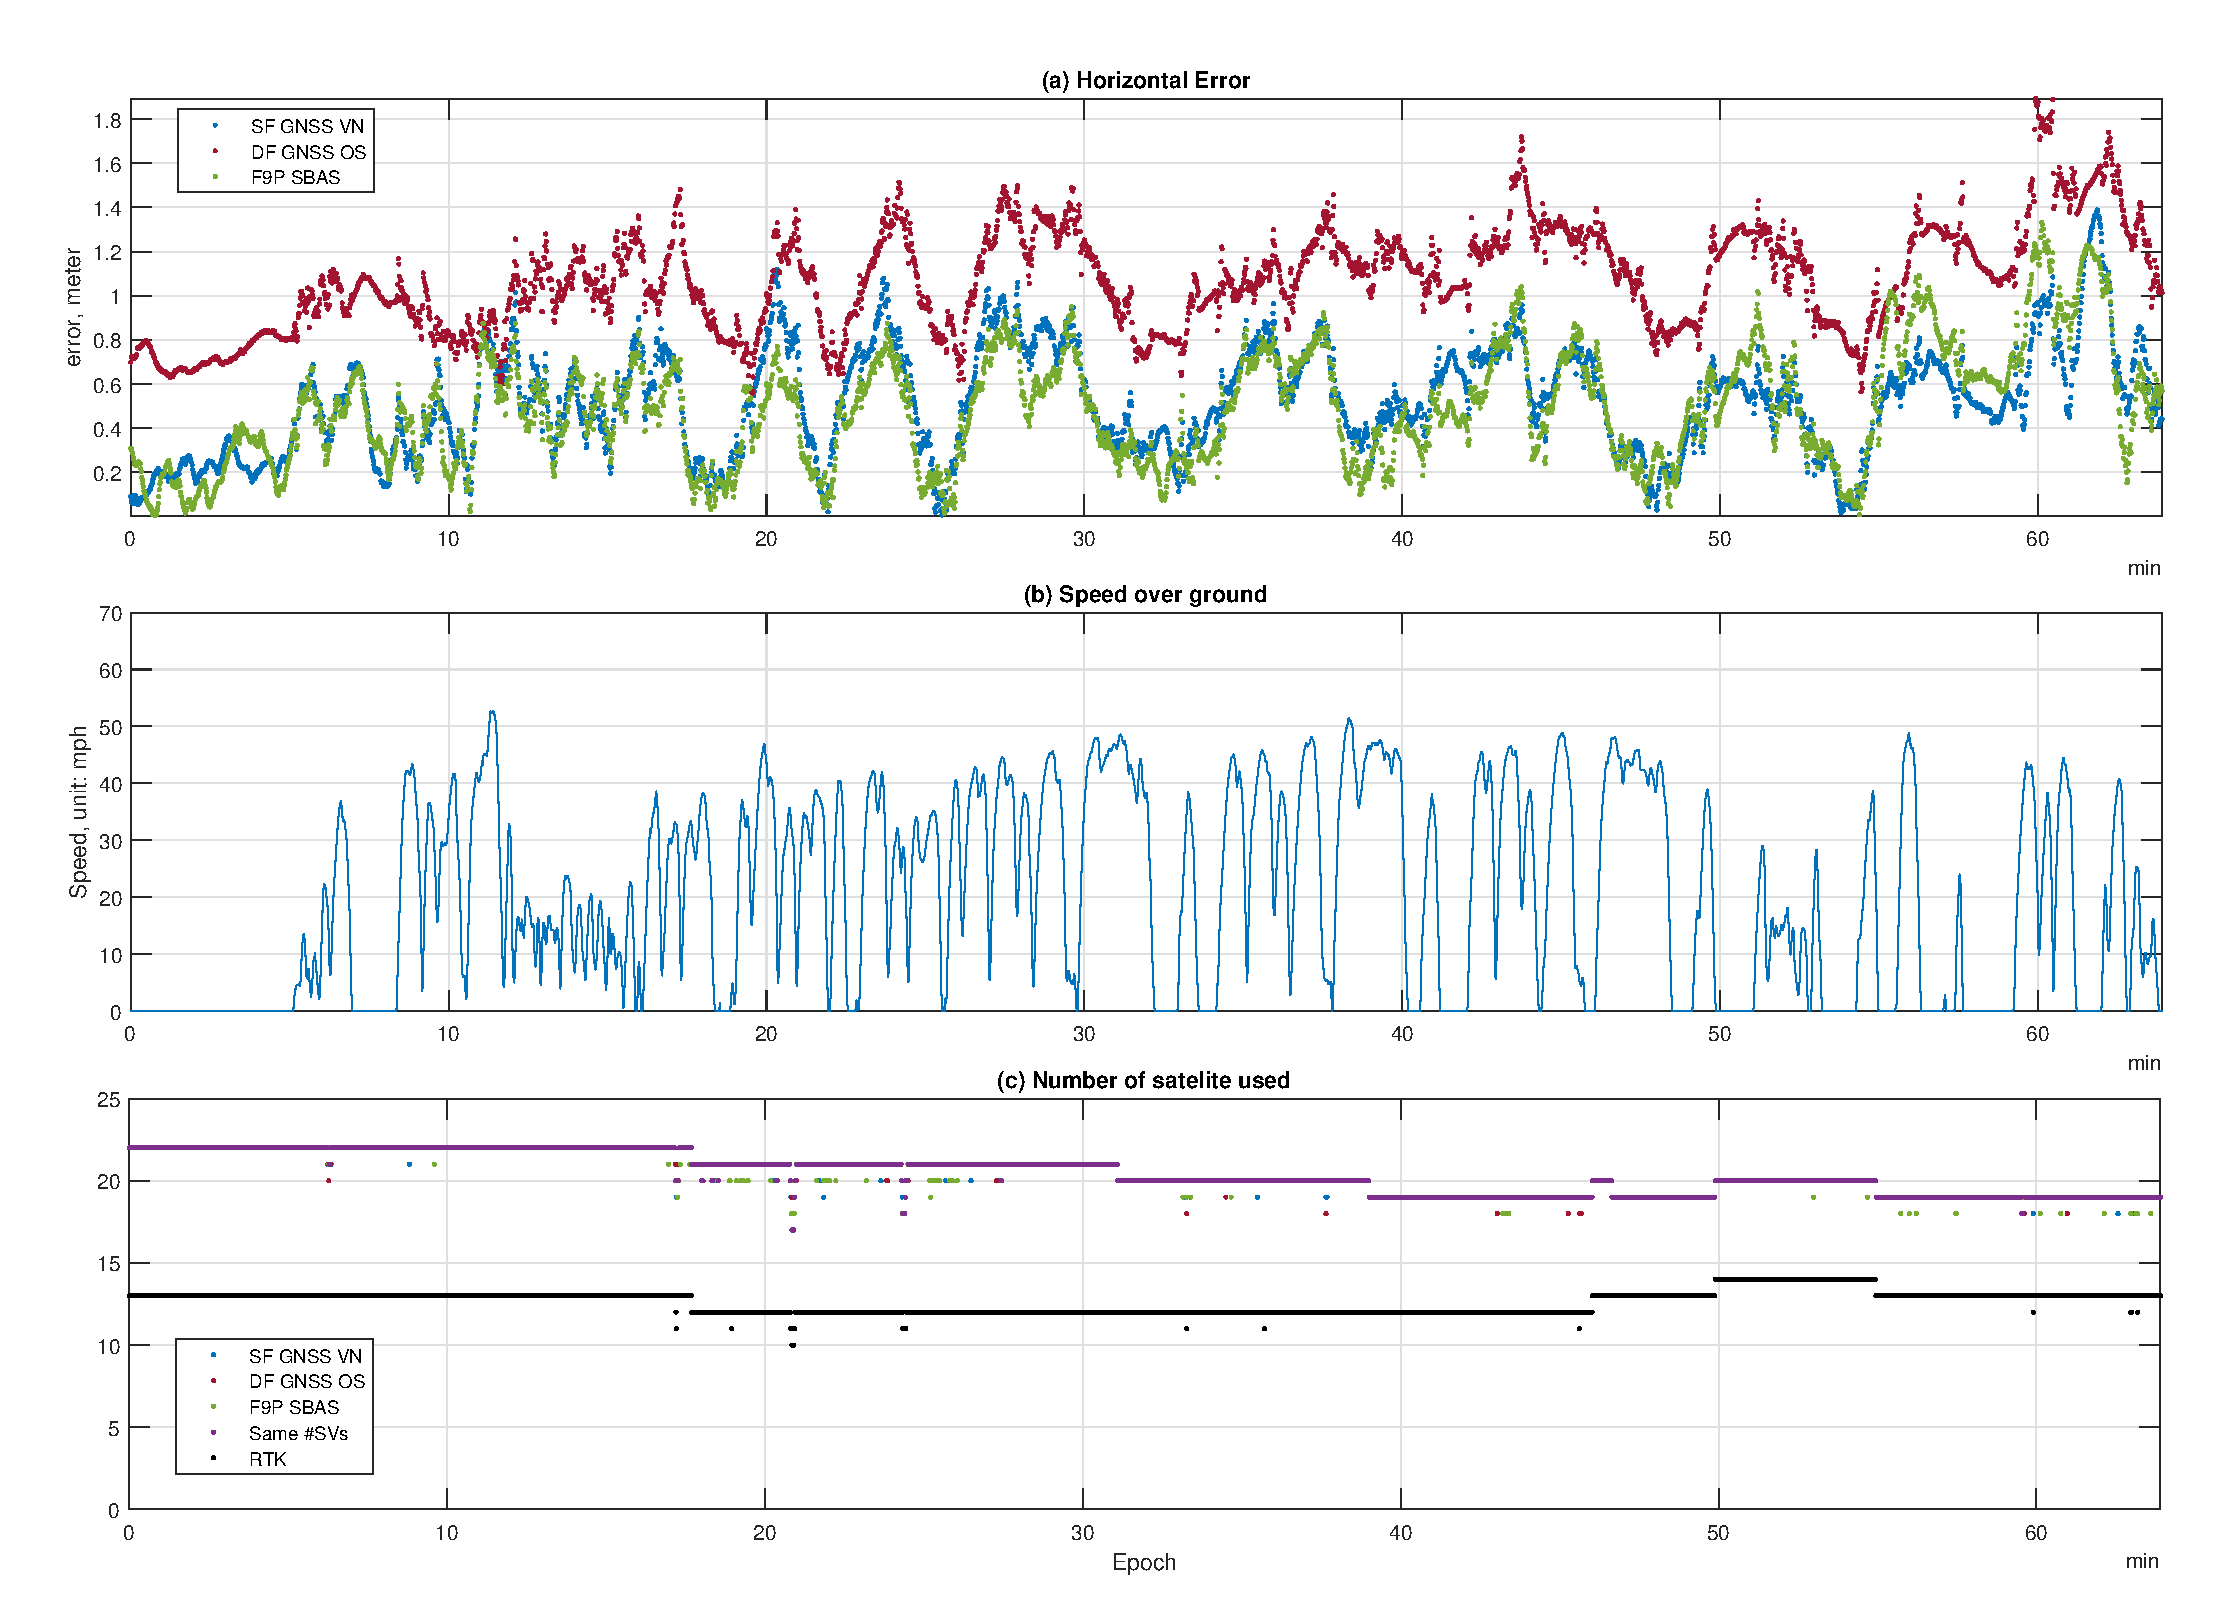
\includegraphics[width=0.9\textwidth]{figures/dynamicinfo_dual.eps}
		\caption{Vehicle speed and number of satellites used for moving test using dual band antenna.}
		\label{fig:m2vspeed}
	\end{figure}
	
	\begin{figure}[H]		
		\centering		
		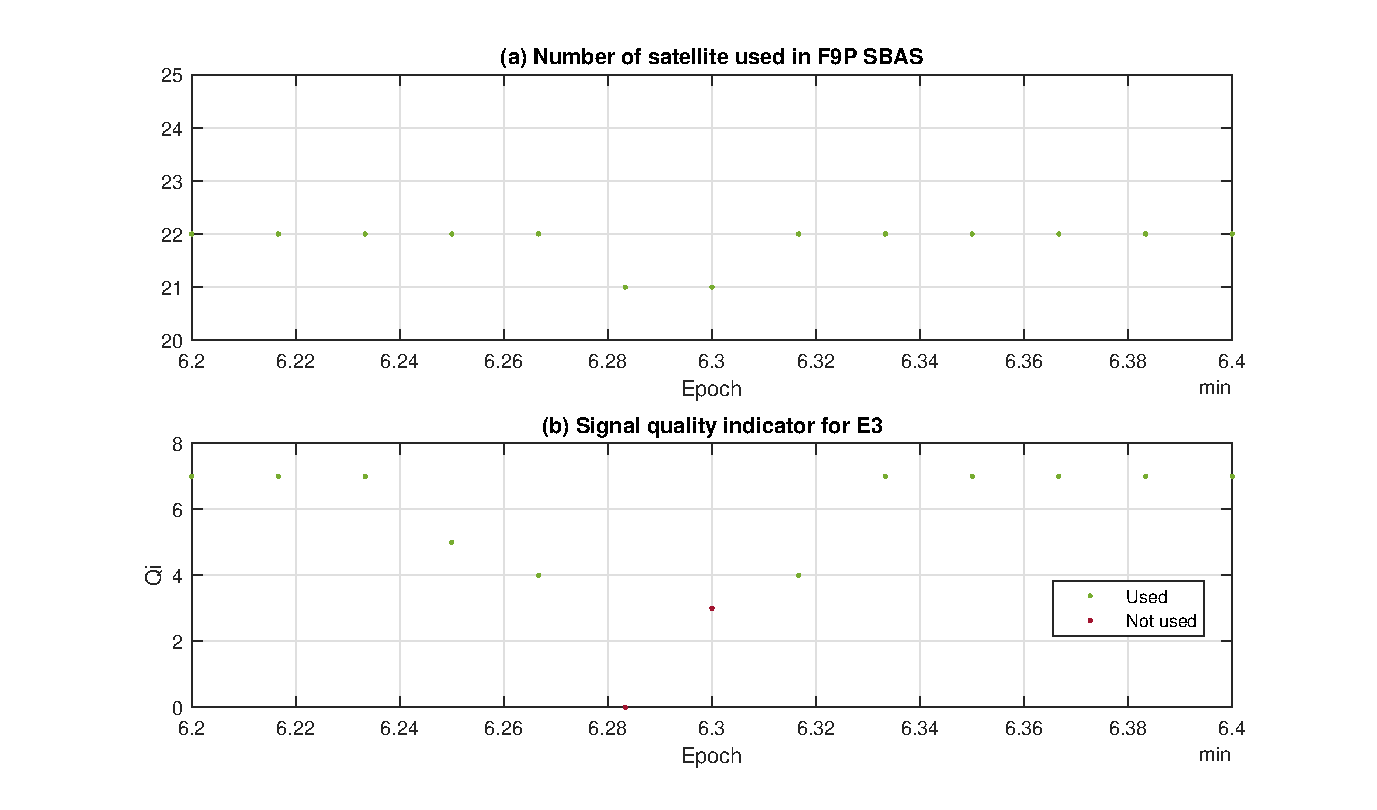
\includegraphics[width=0.9\textwidth]{figures/Qi.eps}		
		\caption{An example of signal quality indicator corresponding to satellite usage status from F9P SBAS in moving test using dual band antenna.}		
		\label{fig:qi}	
	\end{figure}
	
	
	\section{Lane Matching Application}
	This section provide an additional experiment for evaluating the VN-DGNSS in an lane matching application. 
	The goal is that the software uses the receiver computed position to determine in which lane the vehicle is situated as it drives along the lane. The system level traffic or intersection controllers can use this lane inventory information to more efficiently control roadway 
	management. Correct lane determination is a function of position estimation accuracy. This evaluation compares application performance for two receivers one with SF GPS VN using VN-DGNSS corrections and the other with SF GPS SPS.
	
	\subsection{Hardware Setup}
	This moving test using two u-blox M8P single-frequency receivers. 
	One communicated with the UCR VN-DGNSS server, while another one operated in SPS mode, without 
	external corrections. A third u-blox ZED-F9P dual-frequency receiver operated in RTK integer fixed solution to provide a centimeter level accuracy solution that was used as the ground truth trajectories.
	
	\subsection{Experiment Description}
	In this experiment, we drove a sedan on a customized road tesbted inside the UCR CE-CERT parking lot that contained two lanes each 3.6 meters wide. The length of road testbed is about 270 meters. The vehicle was driven along both lanes three times in each direction yielding a total of 12 lane traverses, as show in Fig. \ref{fig:LDsk}.
	The antenna (red circle) was mounted on the roof of the sedan (blue box) at three different locations for the purpose of simulating driving at different lateral positions relative to the lane center line. The green arrows indicate 6 straight driving tests from West to East direction and East to West direction, respectively. 
	\begin{figure}[H]		
		\centering		
		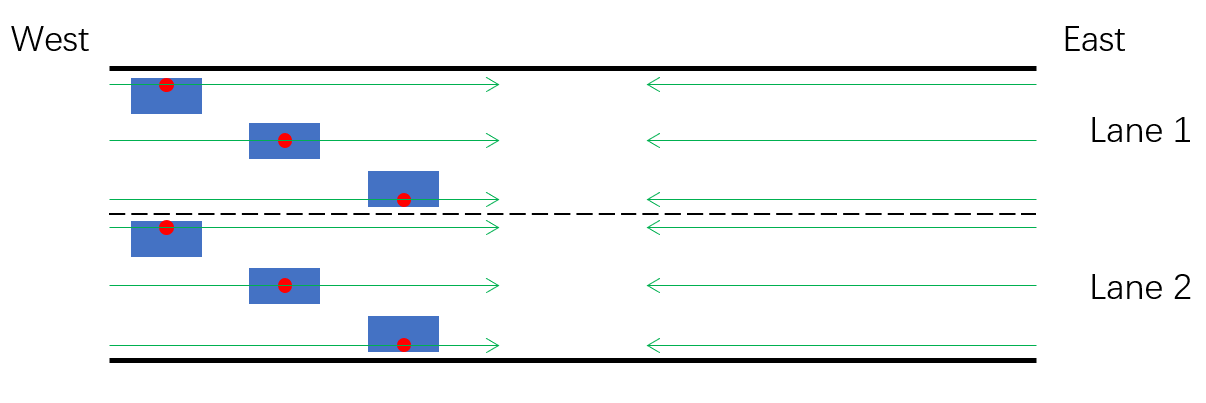
\includegraphics[width=0.9\textwidth]{figures/LDsketch.png}	
		\caption{Sketch of the lane determination driving test.}		
		\label{fig:LDsk}	
	\end{figure}
	
	\subsection{Experimental Results}
	Fig. \ref{fig:e2w} and Fig. \ref{fig:w2e} show the trajectories of the 12 lane traverses. The red curves show the ground truth trajectory. The green curves show the trajectory computed 
	by the M8P receiver using SF GPS VN. The blue curves show the trajectory computed by the M8P receiver using SF GPS SPS. 
	Fig. \ref{fig:e2w} shows trajectories driving from East to West. Fig. \ref{fig:w2e} shows trajectories driving West to East. The red trajectory shows the correct lane determination, with the first three traverses in the bottom lane (southern) and the last three traverses in the top lane (northern).
	
	Fig. \ref{fig:e2w} and Fig. \ref{fig:w2e} allow the reader to visually see whether the SF GPS VN and SF GPS SPS computed positions are in the correct lane. It is clear that the SF GPS VN trajectories are closer to the ground truth RTK solution than are the SF GPS SPS
	trajectories. The SF GPS VN trajectories are also more frequently in the correct lane. Only in the last graph in Fig. \ref{fig:w2e} does the green curves surpass the edge of upper lane.
	\begin{figure}[H]		
		\centering		
		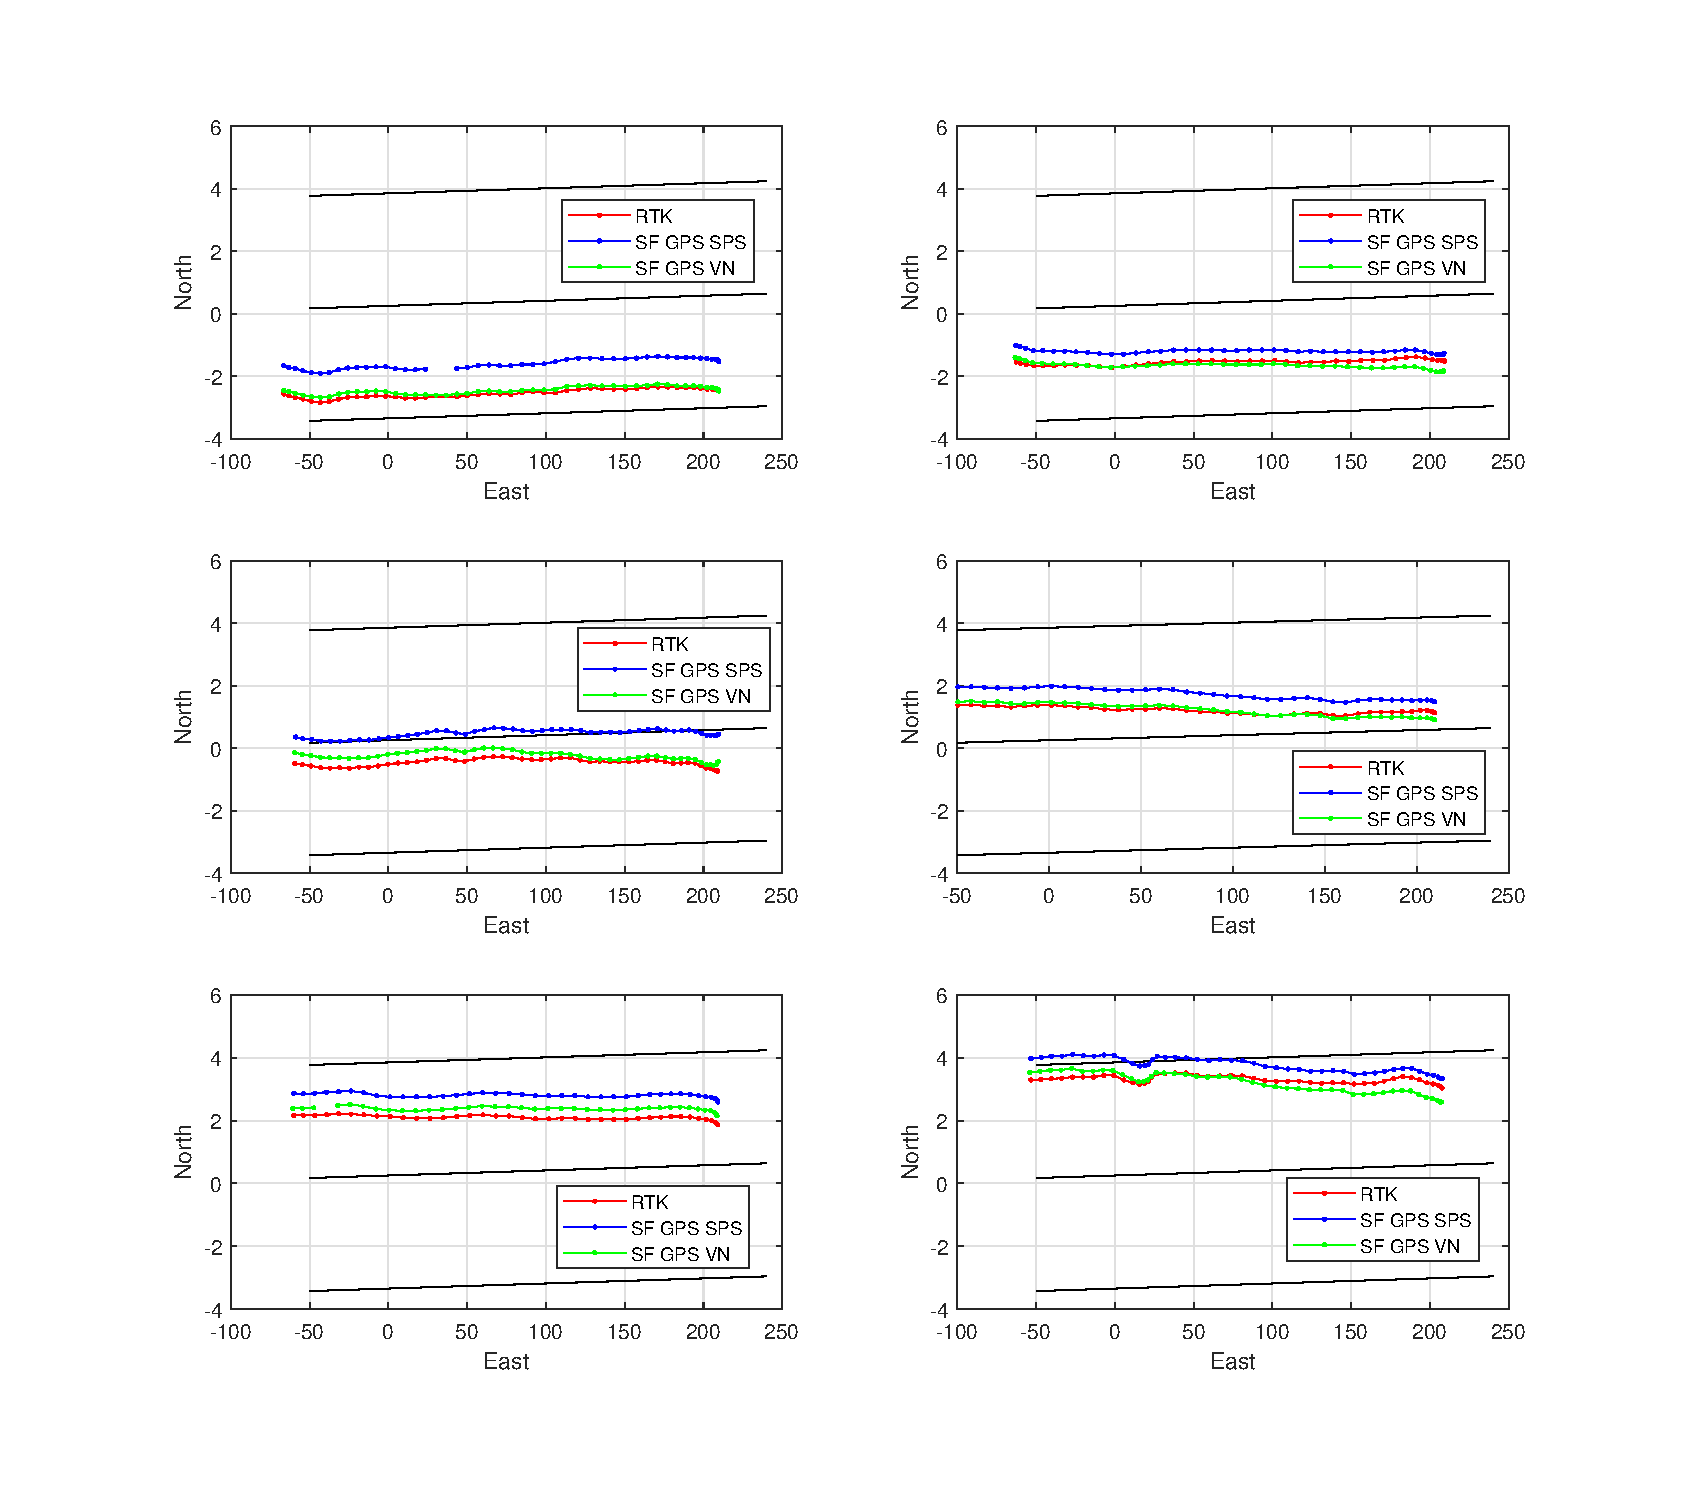
\includegraphics[width=0.9\textwidth]{figures/e2w.eps}		
		\caption{Trajectory of East to West direction driving test.}		
		\label{fig:e2w}	
	\end{figure}

	\begin{figure}[H]		
		\centering		
		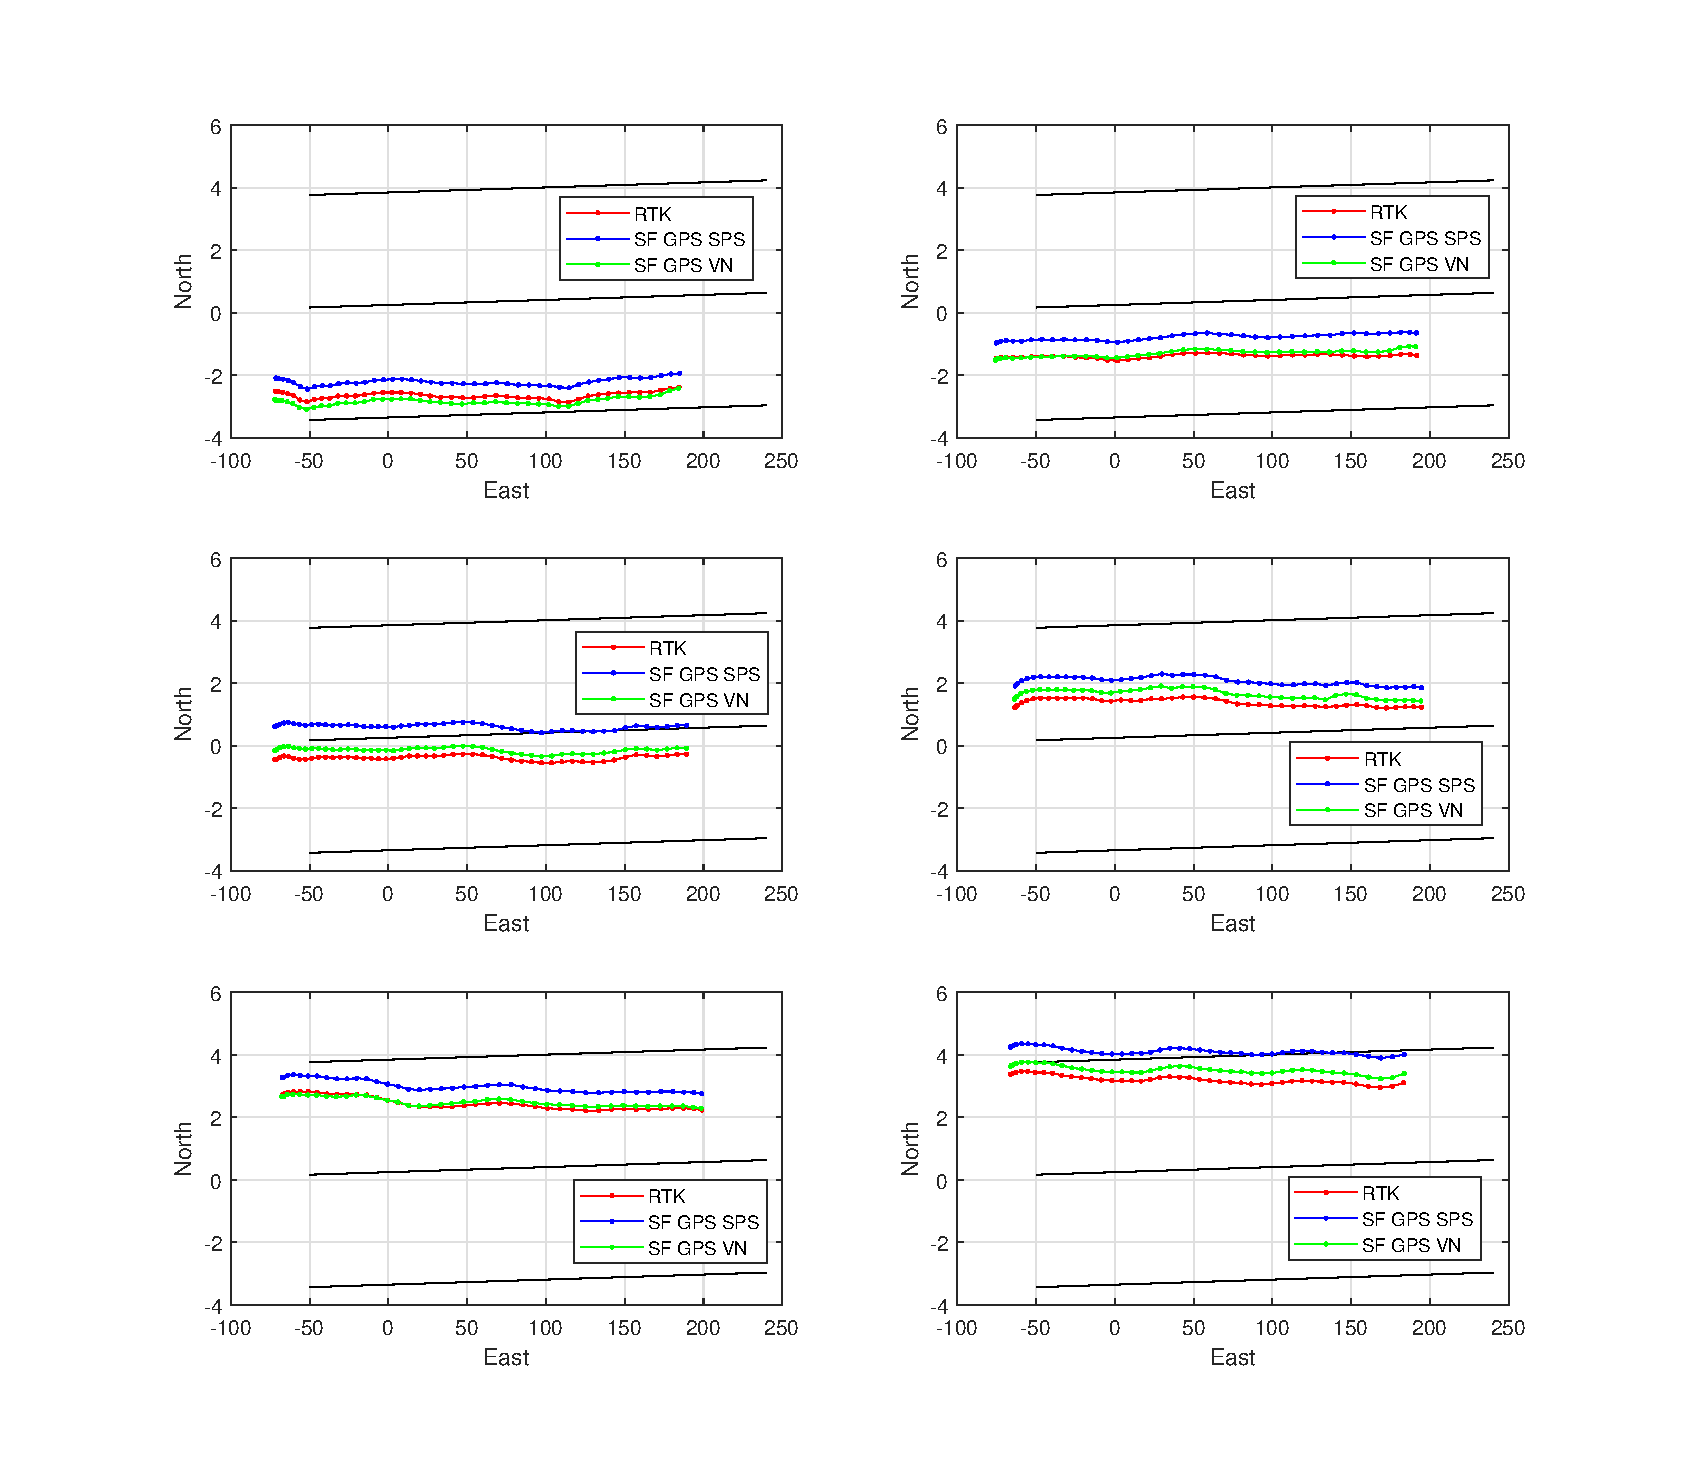
\includegraphics[width=0.9\textwidth]{figures/w2e.eps}	
		\caption{Trajectory of West to East direction driving test.}		
		\label{fig:w2e}	
	\end{figure}
	
	Fig. \ref{fig:probLD} shows the probability of making the correct lane decision using the SF GPS SPS and SF GPS VN positions as a function of the distance of the ground-truth trajectory from the lane center. When the vehicle is near the lane center (i.e., less than 0.5 m), both SF GPS SPS and SF GPS VN correctly determine the lane. As the distance from the lane center line increases, the distance to the lane boundary decreases, so that position error begins to affect the lane determination decision. The decrease in probability of making the correct decision drops off earlier and faster for the SF GPS SPS solution, dropping below 95\% at about 0.7 m, which is 1.1 m from the lane edge. The solution using the UCR VN-DGNSS server maintains correct decision through 1.3 m from the lance center, which is 0.5 m from the lane edge.
	\begin{figure}[H]		
		\centering		
		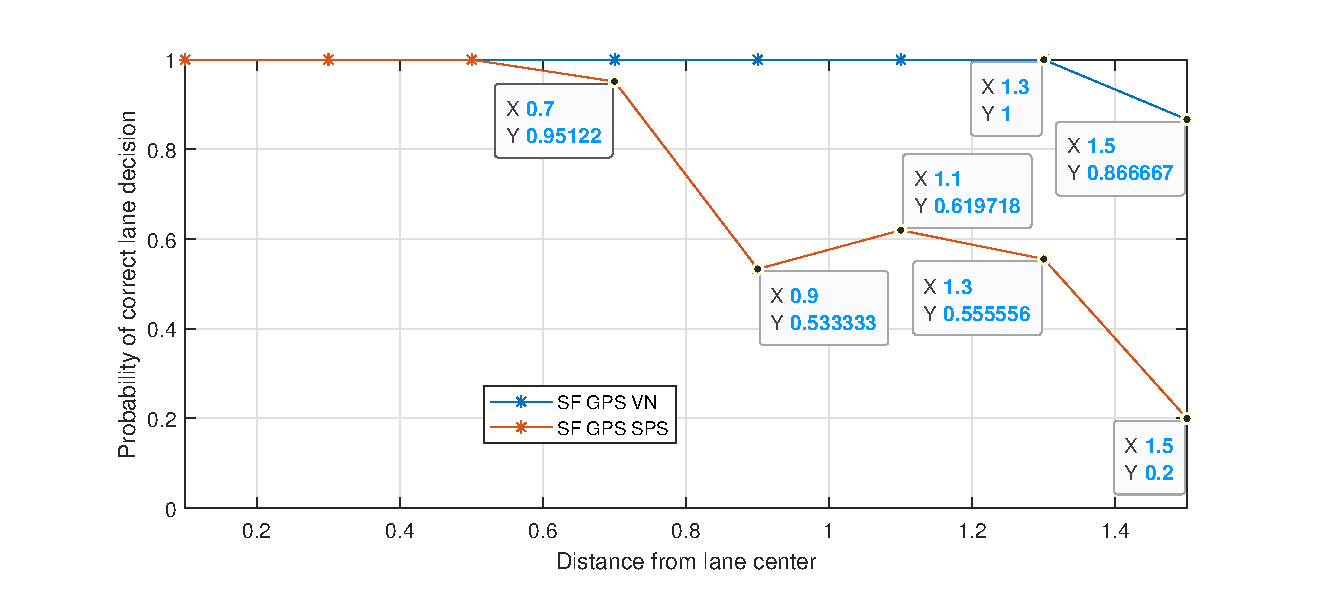
\includegraphics[width=0.9\textwidth]{figures/probLD.eps}	
		\caption{Probability of making the correct lane decision.}		
		\label{fig:probLD}	
	\end{figure}

	\bibliographystyle{ieeetr}
	\bibliography{References.bib}
	
\end{document}